%%%%%%%%%%%%%%%%%%%%%%%%%%%%%%%%%%%%%%%%%%%%%%%%%%%%%%%%%%%%%%%%%%%%%%%%%%%%%%%
% name:         | network.tex
% @uthor:       | Charles Gueunet
% title:        | Include : Le protocole TCP/IP
% brief:        | Explication du protocole TCP/IP
% licence:      | free
% more:         | Warning: inputenc en utf8
%               | Warning: n'oublies pas vos \subsection (3 à 4 maximum)
%%%%%%%%%%%%%%%%%%%%%%%%%%%%%%%%%%%%%%%%%%%%%%%%%%%%%%%%%%%%%%%%%%%%%%%%%%%%%%%


% modele dod : explication de Reseau -> Application
% image modele dod

% Reseau : Ethernet / Bluetooth ...
% Internet : IP addresse (6-4) - ICMP , IGMP
% Transport : Protocol -- TCP / UDP (rapide) - /etc/services  : lien service port protocol
% Application : La donnee, communication noeud à noeud

% Bilan avec image detaillant les headers

\section{Le protocole TCP/IP}
\subsection{Introduction}
\begin{frame}\frametitle{Introduction}
    {\Huge Le protocole TCP/IP}

    \vspace{2em}

    Le net c'est bien, mais comment les machines communiquent ?
\end{frame}


% Presentation du modele DoD dans sa globalité
% Explications rapide des couches (on va revenir dessus en detail en suivant)
% Quelques exemple pour ceux qui connaissent deja
\subsection{Le modèle DoD}
\begin{frame}\frametitle{}
    {\Huge Présentation du modèle DoD}

    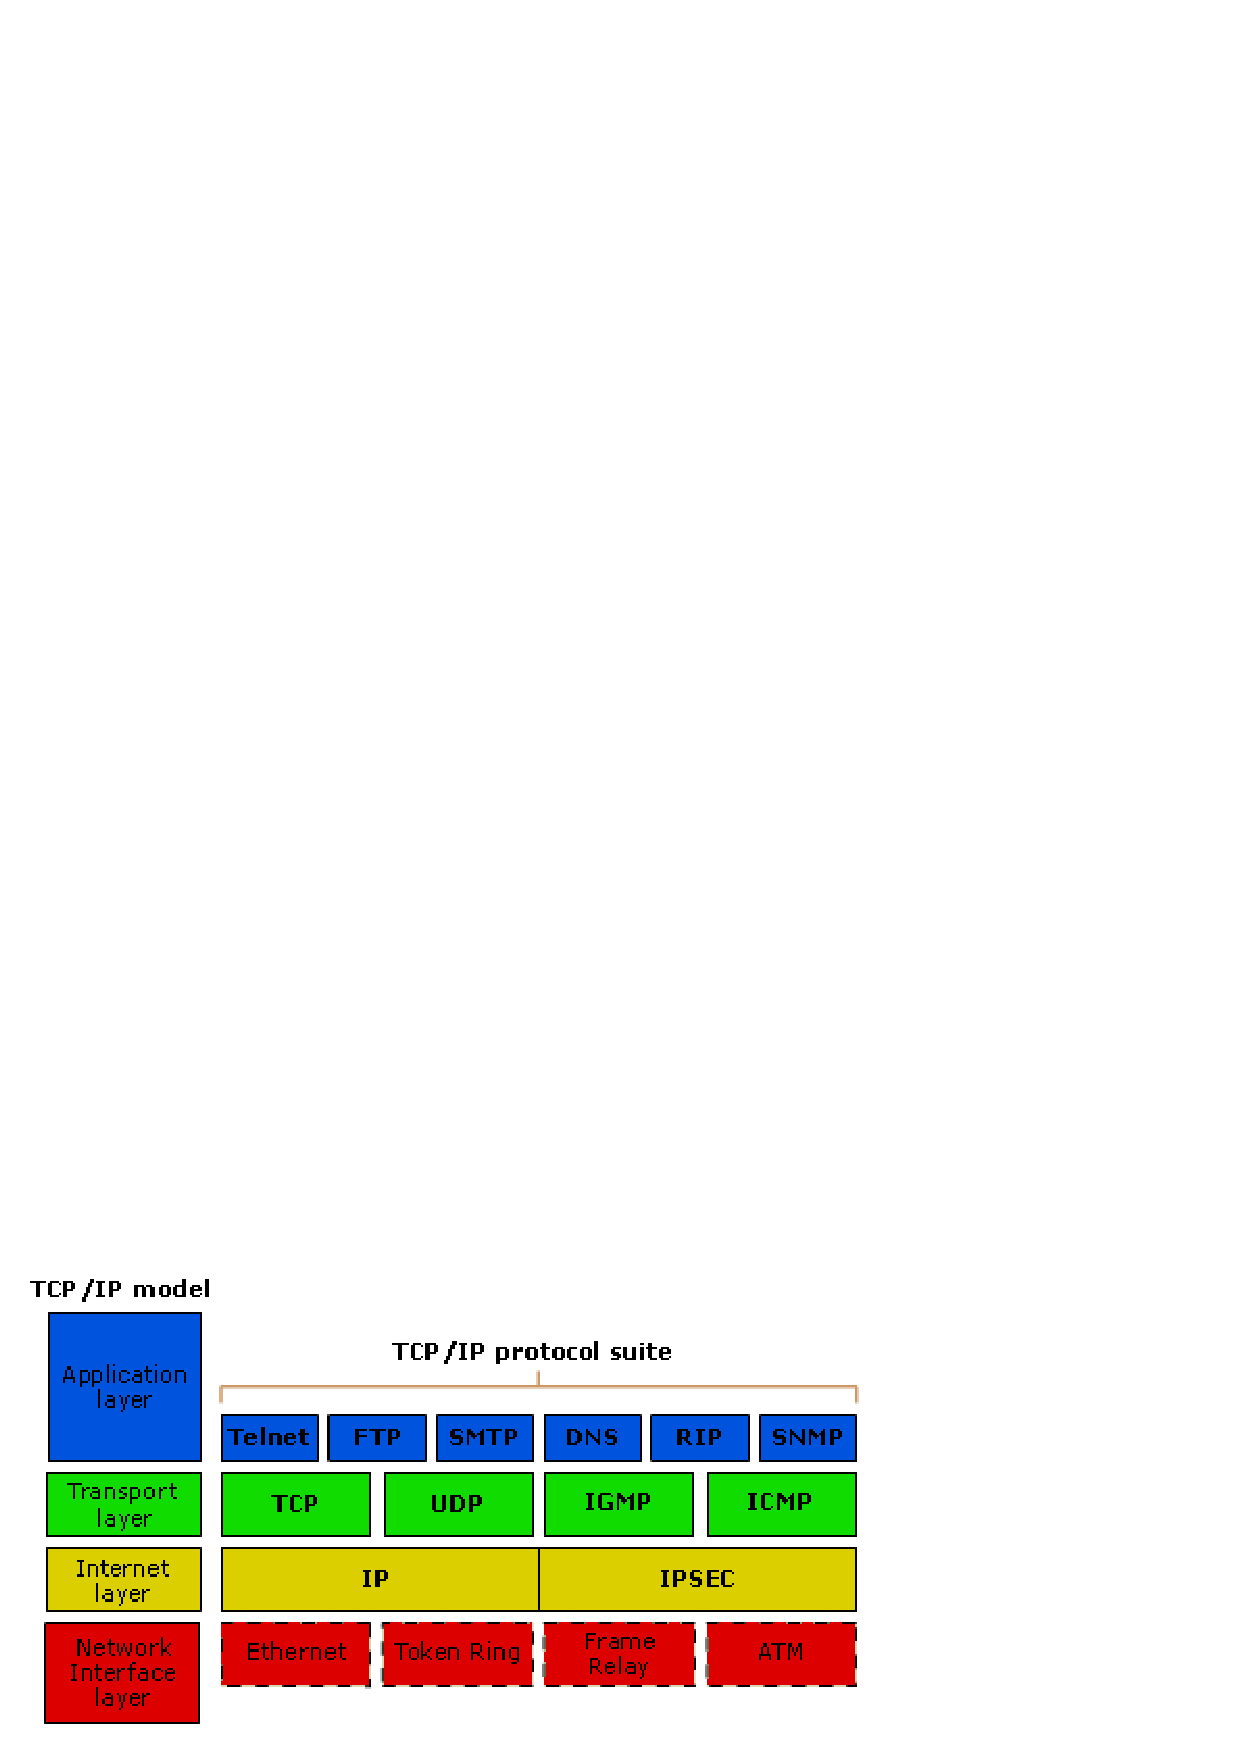
\includegraphics[scale=0.75]{res/DodModel.pdf}

\end{frame}


% Couche réseau : Niveau Hardware, la facon dont les 
% donnée sont acheminée entre deux machines (niveau MAC)
\begin{frame}\frametitle{Couche réseau}

    \begin{itemize}
        \item \textbf{{\Large Couche réseau}: Niveau physique}
    \end{itemize}
     
    % Durant explication : dessin tableau de deux PC relié

\end{frame}


% La couche internet : Interconnexion de reseau (mode déconnecté)
% Sert à l'adressage et au routage des packets
% En d'autre terme l'acheminement de packet à traver plusieurs machines
% niveau IP
\begin{frame}\frametitle{Couche internet}

    \begin{itemize}
        \item {\Large Couche réseau}: Niveau physique
        \item \textbf{{\Large Couche internet}: Adressage et routage des packets}
    \end{itemize}

    % Durant explication : dessin tableau de deux PC reliés avec des intermediaires
    % -> Illustre le routage et l'adressage

\end{frame}


    %%%%%%%%%%%%%%%%%%%%%%%% EXEMPLE / EXERCICE
    %% TP avec nc : defaut  - Protocol enttec
    %% Une Demo avec tcpdump (basé sur les manip du TP)

    %%%%%%%%%%%%%%%%%%% TP %%%%%%%%%%%%%%%%%%%%%

    % Sur le PC serveur :
    %    for i in {prisDeb..priseFin}; do nc -l -p $i; done
    % Et aussi
    %    tcpdump -A -i lo   # a ameliorer pour visu des ports
    %    On voit le TCP : Envoie - reponse OK
    % 
    % Chacun avec son num de prise se connecte 
    %
    %%%%%%%%%%%%%%%%%%%%%%%%%%%%%%%%%%%%%%%%%%%%%






% La couche transport : Transmition des données, correction des erreures
% Choix du mode UDP / TCP ( on ne parlera ici que de ces deux la )
% Difference UDP / TCP
\begin{frame}\frametitle{Couche transport} % egalement Host to Host layer

    \begin{itemize}
        \item {\Large Couche réseau}: Niveau physique
        \item {\Large Couche internet}: Adressage et routage des packets
        \item \textbf{{\Large Couche transport}: Transmission des données}
    \end{itemize}

    % Explique succintement les differences TCP/UDP :
    %    TCP         UDP
    % connecté      non connecté
    % ordonné       non ordonné
    % checsum       checksum

\end{frame}


% La couche application : Niveau utilisateur, 
% Echange entre applications
% Choix du protocol à utiliser (généralement TPC/UDP)
\begin{frame}\frametitle{Couche application}

    \begin{itemize}
        \item {\Large Couche réseau}: Niveau physique
        \item {\Large Couche internet}: Adressage et routage des packets
        \item {\Large Couche transport}: Transmission des données
        \item \textbf{{\Large Couche application}: niveau utilisateur}
    \end{itemize}

\end{frame}


% On fait un bilan de chaque couche et de leurs interactions
% Conclusion de la partie modele Dod
\begin{frame}\frametitle{Bilan}

    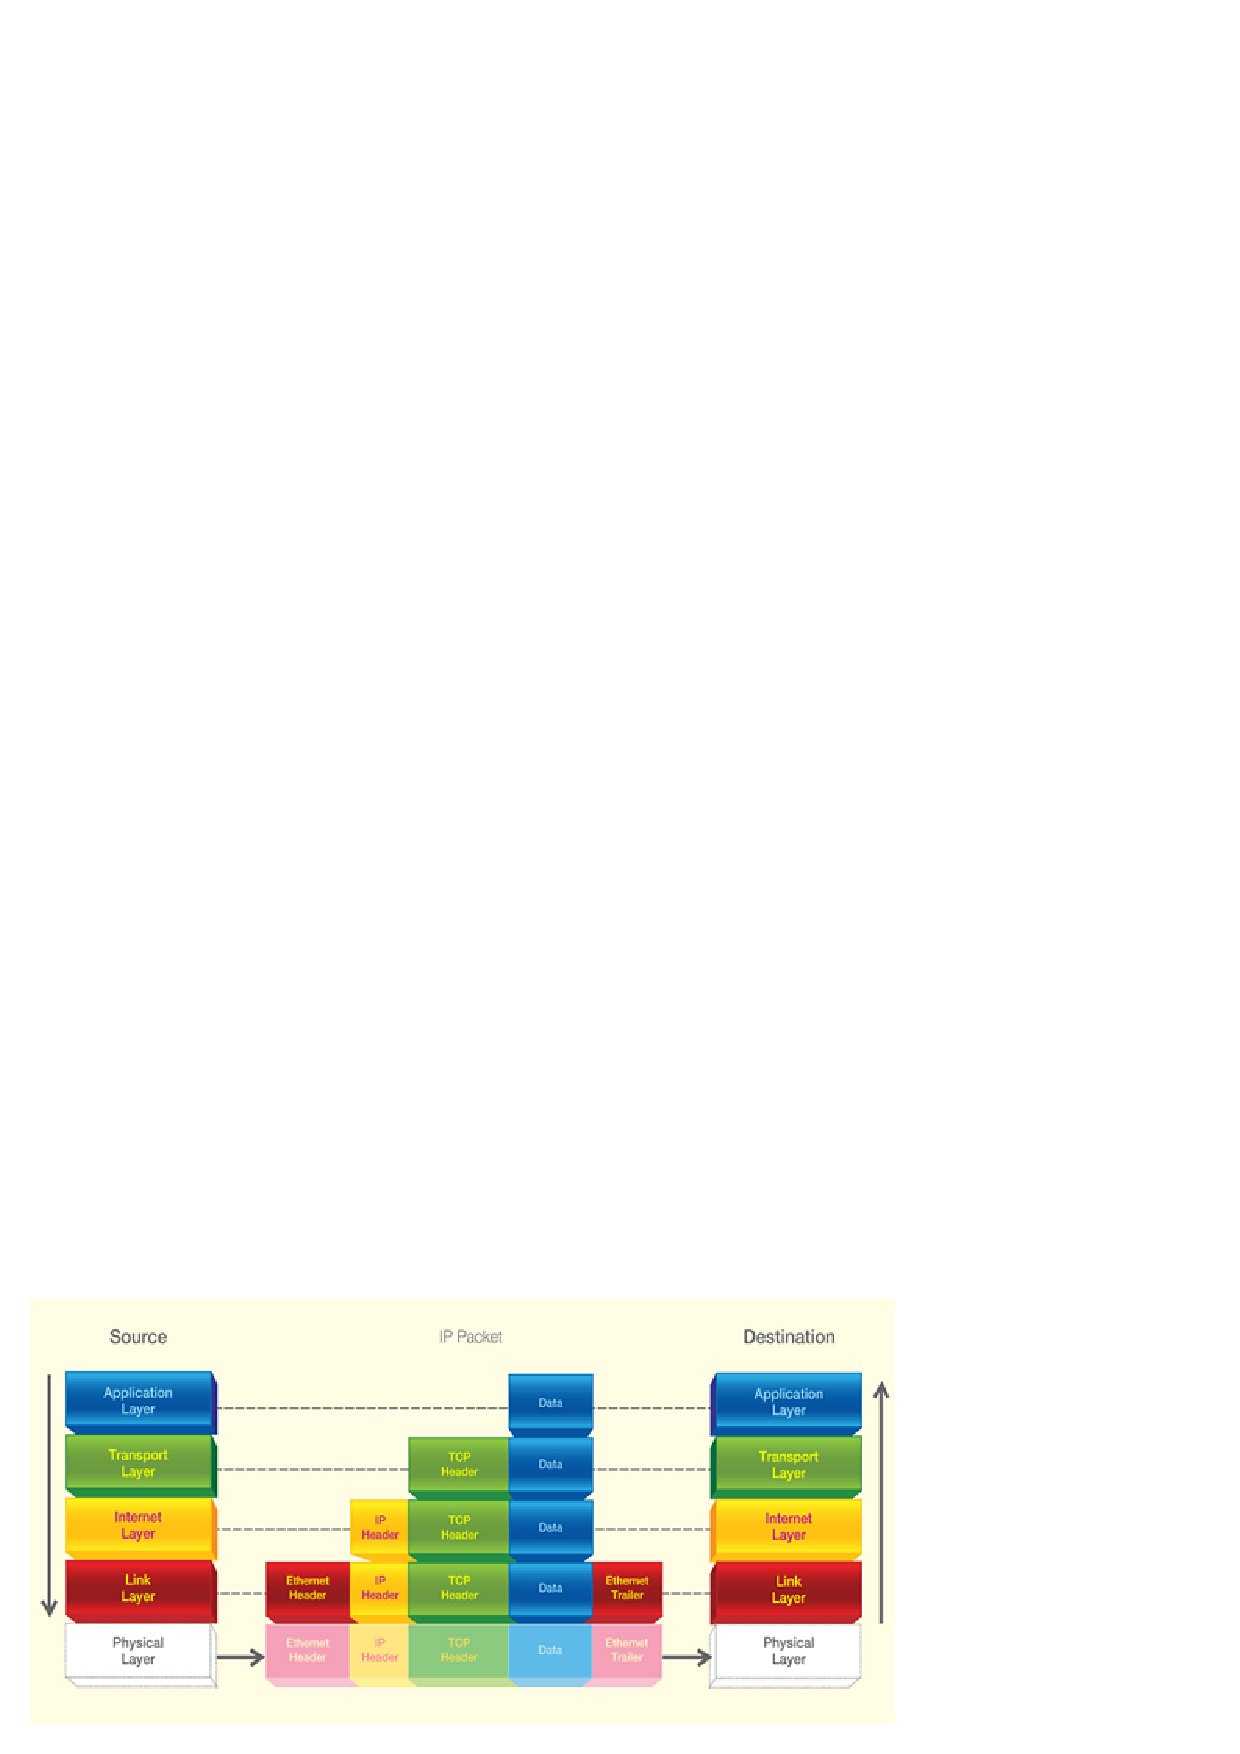
\includegraphics[scale=0.75]{res/DodExplain.pdf}

\end{frame}

% Classes IP : prérequis pour le routage des paquets
\subsection{Classes IP}
\begin{frame}\frametitle{Classes IP}

    \begin{itemize}
        \item {\Large Introduit pour pallier le manque d'adresse IPv4}
        \item {\Large Il y a 5 classes d'adresses}
    \end{itemize}

\end{frame}


% Explication de ce qu'est un masque
\begin{frame}\frametitle{Classes IP}

    \includegraphics[scale=0.6]{res/classes-adresses-ipv4.pdf}

\end{frame}

%
\begin{frame}\frametitle{Classes IP}
    
\begin{table}[h]
\begin{tabular}{l|l|l|l}
Classe & Adresse de sous-réseau   & nb domaine     & nb machine/domaine   \\ \hline
    A  & de 0.0.0.0 à 9.0.0. 0    & 10             & 16 millions           \\ \hline
    A  & 10.0.0.0                 & \multicolumn{2}{l}{réseaux privé}       \\ \hline
    A  & de 11.0.0.0 à 126.0.0.0  & 116            & 16 millions             \\ \hline
    A  & 127.0.0.0                &\multicolumn{2}{l}{loopback}               \\ \hline
    B  & de 128.0.0.0 à 191.0.0.0 & 16 mille       & 66 mille                  \\ \hline
    A  & 192.168.0.0              & \multicolumn{2}{l}{réseaux prive}           \\ \hline
    A  & 192.0.0.0                & \multicolumn{2}{l}{cas particulier}           \\ \hline
    C  & de 193.0.0.0 à 223.0.0.0 & 2 millions     & 256                         \\ \hline
    D  & de 224.0.0.0 à 239.0.0.0 &\multicolumn{2}{l}{groupe de multicast}        \\ \hline
    E  & de 240.0.0.0 à 255.0.0.0 &\multicolumn{2}{l}{réservé pour usage futur}    \\ 
\end{tabular}
\end{table}

\end{frame}

% Partie routage
\subsection{Routage}
\begin{frame}\frametitle{Le routage}

    {\Huge Comment une machine fait-elle transiter un paquet ?}\\
    Retour sur les chouches réseau et internet\\
    

\end{frame}

% Cas simple, sur un meme reseau
% Le paquet va de A a B, que fait le routeur
% Principe du routage
\begin{frame}\frametitle{Le routage}

        \begin{minipage}{0.35\textwidth}
            \begin{figure}[H]
                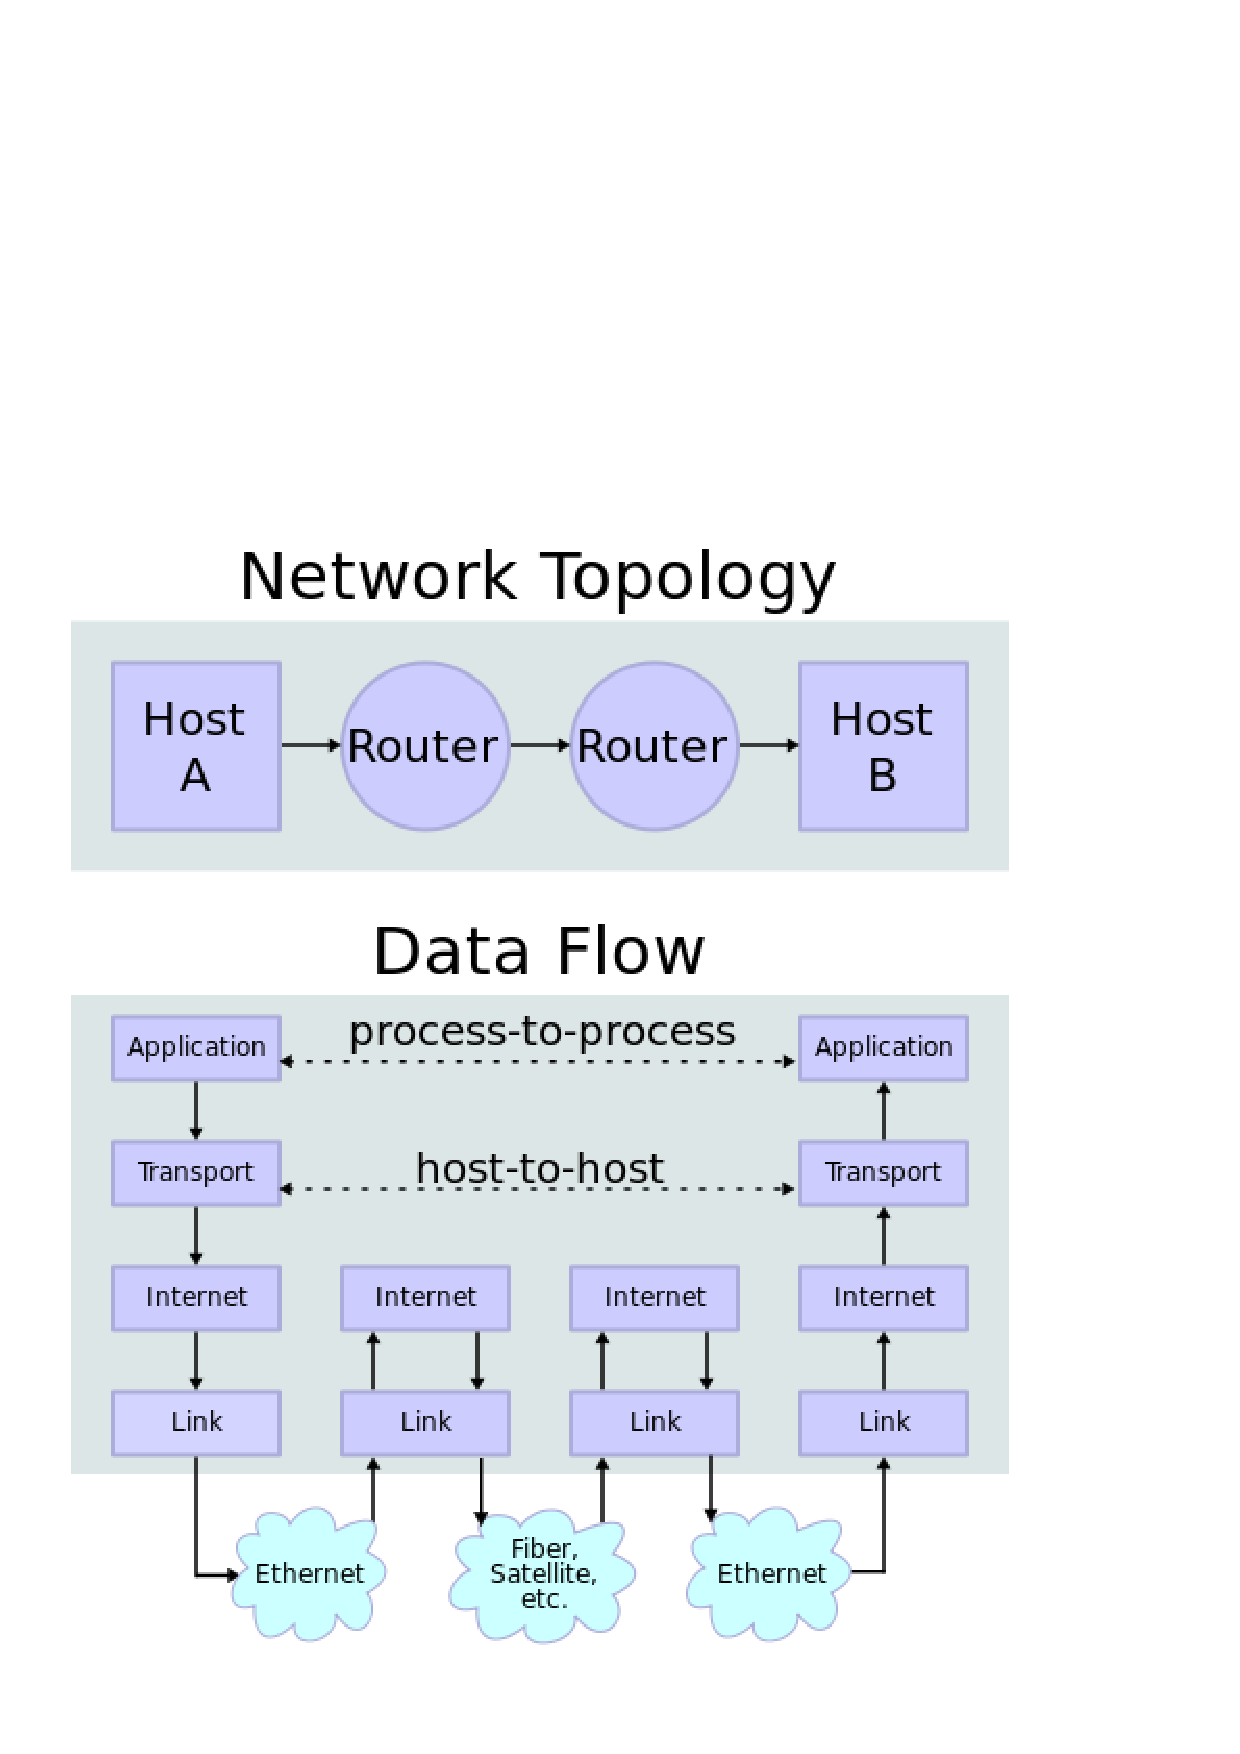
\includegraphics[scale=0.35]{res/DodConnect.pdf}
            \end{figure}
        \end{minipage} \hfill
        \begin{minipage}{0.5\textwidth}
            {\color{red}Host A: ip=\$ipA, MAC:\$macA}\\
            {\color{green}Host B: ip=\$ipB, MAC:\$macB}\\
             Paquet A -> B, Que fait le Routeur:
            \begin{itemize}
                \item Il recoit un paquet de {\color{red}\$macA}
                \item Il lit la destiniation{\color{green}\$ipB}
                \item Il cherche dans sa table de routage à qui transmettre
                \item Il envoie le paquet à {\color{green}\$macB}
            \end{itemize}

        \end{minipage}

\end{frame}


% Cas simple, routage inter reseau
% Table de routage
\begin{frame}\frametitle{Le routage}

    \begin{figure}[H]
        \includegraphics[scale=0.35]{res/routageIP_1.png}
    \end{figure}
    Table de routage :
    \begin{table}[h]
        \begin{tabular}{l|l|l|l}
Destination   & Masque ss réseau  & Paserelle     & Interface   \\ \hline
192.168.10.0  & 255.255.255.0     & 192.168.10.99 & 192.168.10.99\\ \hline
192.168.20.0  & 255.255.255.0     & 192.168.20.99 & 192.168.20.99\\ \hline
192.168.30.0  & 255.255.255.0     & 192.168.30.99 & 192.168.30.99\\ \hline
        \end{tabular}
    \end{table}

\end{frame}


% Cas complexe, routage inter reseau avec intermediaire
% Table de routage
\begin{frame}\frametitle{Le routage}

    \begin{figure}[H]
        \includegraphics[scale=0.35]{res/routageIP_2.png}
    \end{figure}
    Table de routage :
    \begin{table}[h]
        \begin{tabular}{l|l|l|l}
Destination   & Masque ss réseau  & Paserelle     & Interface   \\ \hline
192.168.10.0  & 255.255.255.0     & 192.168.10.99 & 192.168.10.99\\ \hline
192.168.20.0  & 255.255.255.0     & 192.168.20.99 & 192.168.20.99\\ \hline
192.168.30.0  & 255.255.255.0     & 192.168.30.99 & 192.168.30.99\\ \hline
\color{red}192.168.40.0&\color{red}255.255.255.0&\color{red}192.168.30.254&\color{red}192.168.30.99\\
        \end{tabular}
    \end{table}

\end{frame}



